\hypertarget{Introduction}{%
\chapter{Introduction}\label{Introduction}}

\section{Présentation de la structure
d'accueil}

Durant la période de mon stage , j'ai été accueilli au
\textbf{Laboratoire de Mathématiques Informatique et Application
(LAMIA)} de l'Université des Antilles (UA).

Pour présenter cette structure, il me faut tout d'abord présenter
l'université à laquelle il est rattaché.

\hypertarget{luniversite-des-antilles}{%
\subsection{L'université des Antilles}\label{luniversite-des-antilles}}

Bien que ce soit l'université dans laquelle j'ai fait toutes mes études,
voici quelques chiffres que je ne connaissais pas et qui donnent la
mesure de sa taille :

L'Université des Antilles s'organise autour deux pôles universitaires
régionaux autonomes : le « Pôle Guadeloupe » et le « Pôle Martinique ».

Sur ces pôles, l'Université assure des missions d'\emph{enseignement} et
de \emph{recherche}, assistées par des \emph{administratifs et des
techniciens}.

\hypertarget{administration-et-personnel-technique}{%
\subsubsection{Administration et personnel
technique}
\label{administration-et-personnel-technique}}

l'UA emploie 414 Administratifs et Techniciens (environ 200 personnes
pour l'administation centrale et 100 répartis sur chaque pôle)

\hypertarget{enseignements}{%
\subsubsection{Enseignements}\label{enseignements}}

L'UA délivre des diplomes de la licence au doctorat dans de nombreux
domaines. Au total, cela représente :

\begin{itemize}
\tightlist
\item
  484 enseignants-chercheurs (environ 240 pour chaque pôle)
\item
  12 000 étudiants (environ 7000 pour la Guadeloupe , 5000 pour la
  Martinique)
\end{itemize}

Pour l'informatique, cela représente : - autour de 20
enseignants-chercheurs - autour de 120 étudiants

\hypertarget{recherche}{%
\subsubsection{Recherche}\label{recherche}}

La recherche est structurée en laboratoires auxquels sont rattachés les
enseignants chercheurs qui peuvent former de futurs chercheurs : les
doctorants.

L'université compte ainsi au total :

\begin{itemize}
\tightlist
\item
  17 laboratoires
\item
  320 doctorants
\end{itemize}

Pour ma part, comme signalé précédemment, j'ai effectué mon stage dans
le laboratoire LAMIA que je vais maintenant présenter.

\hypertarget{le-lamia}{%
\subsection{Le LAMIA}\label{le-lamia}}

Le \textbf{Laboratoire de Mathématiques Informatique et Application
(LAMIA)}, comme son nom l'indique, se concentre sur les recherches en
informatiques et mathématiques.

Il compte une soixantaine de membres (Professeurs des Universités,
Maitres de Conférences, ATER, Doctorants) répartis sur deux pôles
(Guadeloupe et Martinique) au sein de trois équipes internes :

\begin{itemize}
\tightlist
\item
  Equipe
  \href{http://lamia.univ-ag.fr/index.php?page=equipe-mathematiques}{\textbf{Mathématiques}
  (analyse variationnelle, analyse numérique, EDP, analyse statistique,
  mathématiques discrètes)} ;
\item
  Equipe Informatique
  \href{http://lamia.univ-ag.fr/index.php?page=equipe-danais}{\textbf{DANAIS}
  : Data analytics and big data gathering with sensors} ;
\item
  Equipe Informatique
  \href{http://lamia.univ-ag.fr/index.php?page=equipe-aid}{\textbf{AID}
  : Apprentissages Interactions Donnees} ;
\end{itemize}

De plus, le LAMIA accueille en son sein un groupe de chercheurs associés
travaillant en Epidémiologie clinique et médecine.

L'équipe avec laquelle il m'a été donné de travailler principalement est
celle d'\textbf{Apprentissages Interactions Données} qui développe des
méthodes de traitements et d'analyse de données hétérogènes : images
(classique, multi-spectrale), séquences vidéos, séries temporelles et
spatio-temporelles, dont la responsable est \textbf{Mme. Hélène
Paugam-Moisy}.

Indépendamment de ces équipes, les travaux de recherche du laboratoire
se répartissent en \textbf{projets} qui peuvent réunir des membres de
plusieurs équipes en \textbf{groupes de travail}. Mon stage était en
fait plus attaché à un projet et un groupe de travail qu'à une équipe.

Ce projet est nommé de façon informelle projet \textbf{``Spikes''} et
concerne l'utilisation de \textbf{réseaux de neurones impulsionnels}
pour l'apprentissage automatique (ces notions seront définies plus
loin). Le groupe de travail associé réunit à l'heure actuelle :

\begin{itemize}
\tightlist
\item
  1 Professeur des Universités
\item
  2 MCF avec HDR
\item
  3 MCF
\item
  1 ingénieur d'études.
\end{itemize}.

C'est avec ces personnes que j'ai travaillé tout au long du stage et mes
tuteurs de stage était \textbf{M.~Vincent PAGÉ et M. ~Manuel CLERGUE}.

Ci dessous, un schéma présentant la structure du laboratoire mon
rattachement à cette structure. (L'équipe de travail \textbf{Spikestrain}
étant informelle, elle ne figure pas sur ce schéma.)

\begin{figure}[h!]
\centering
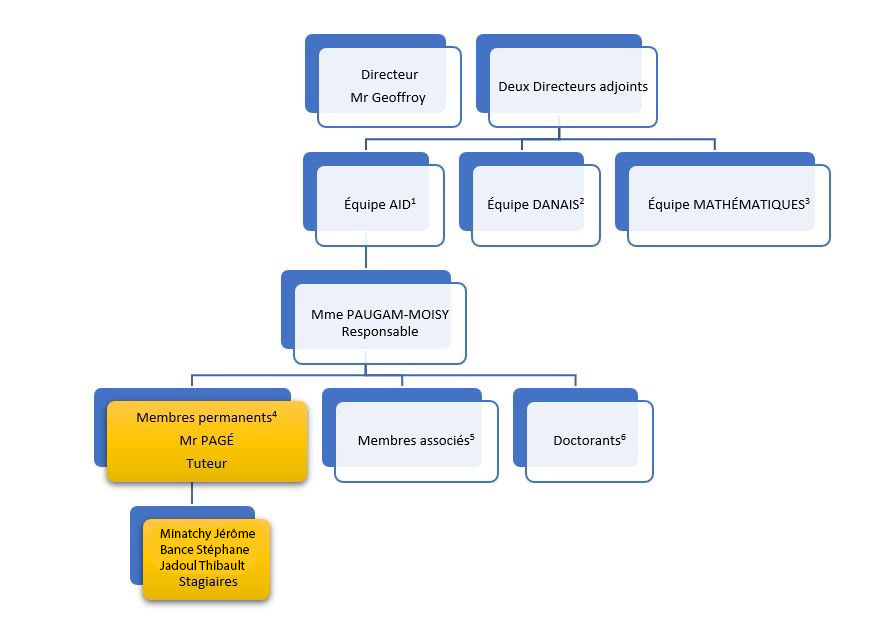
\includegraphics[width=10cm]{./images/orga.jpg}
\caption{Figure 1 Schéma de l'organisation interne du LAMIA:
¹Apprentissages Interactions Données. ²Data analytics and big data
gathering with sensors. ³Mathématiques (analyse variationnelle, analyse
numérique, EDP, analyse statistique, mathématiques discrètes). ⁴Membres
permanents : Suzy Gaucher-Casalis~(MCF),~Enguerran
Grandchamp~(MCF--HDR),~Jean-Luc Henry~(MCF),~Jimmy Nagau~(MCF),~Vincent
Pagé(MCF),~Helene Paugam Moisy~(PR),~Sébastien Régis~(MCF),~Céline
Rémi~(MCF).}
\end{figure}

La prochaine section sera consacrée à la présentation de la thématique
de recherche du groupe ``Spikes'' et de mon stage.


\hypertarget{Objectif_Spike}{%
\section{Objectifs du groupe Spiketrain}\label{Objectif_Spiketrain}}

Le groupe \textbf{Spikestrain} s'intéresse aux techniques
d'\textbf{Intelligence Artificielle}, plus spécifiquement à
l'\textbf{apprentissage automatique} dont l'objectif est de créer des
programmes capable d'apprendre à partir de bases d'exemples.

Actuellement, parmi les techniques permettant l'apprentissage
automatique , une se démarque et est très populaire : les
\textbf{réseaux de neurones artificiels} , notamment dans leur version
\emph{profonde} qui sont très utilisé par exemple par \textbf{Facebook™}
pour sa \textbf{reconnaissance faciale} ou encore par \textbf{Google™}
pour ses \textbf{robots} qui apprennent par \textbf{répétitions} à jouer
(échecs, Go).

\hypertarget{ruxe9seaux-de-neurones-classiques-et-impulsionnels}{%
\section{Réseaux de neurones classiques}\label{ruxe9seaux-de-neurones-classiques}}

Ces réseaux de neurones artificiels sont nés dans les années 1960 et les
techniques d'apprentissage arrivent à maturité seulement maintenant,
avec des résultats très impressionnants.

Bien que basés de façon lointaine sur des neurones biologiques, ils sont
en fait très peu plausibles biologiquement (les neurones échangent des
chiffres entre eux, les informations se rétropropagent\ldots{})


\hypertarget{problematique}{%
\section{Problématique: Classifier les Cachalots}\label{problematique}}

Le challenge "Dyni Odontocete Click Classification, 10 species [ DOCC10 ]
by Universite de Toulon" (https://challengedata.ens.fr/challenges/32) consistait simplement à réaliser un classifieur qui classe les cachalots en une dizaine d'especes à partir de leurs "Clics" pour celà nous avions a disposition une base d'apprentissage labelisée ainsi qu'une base de test non labelisée sur laquelle nous pouvions évaluer les performances réelles de nos classifieurs. Pour cela nous labelision les exemples de la base de test puis envoyions nos prédictions sur le site du challenge qui nous renvoyais nos performances ainsi qu'un classement des performances de tous les participants.

Les deux bases sont consititués d'enregistrements audios des clics des différentes especes de cachalots que je présenterais plus en détail dans la partie analyse des données.
